%% LyX 2.0.6 created this file.  For more info, see http://www.lyx.org/.
%% Do not edit unless you really know what you are doing.
\documentclass[english]{article}
\usepackage[T1]{fontenc}
\usepackage[utf8]{luainputenc}
\usepackage{graphicx}
\usepackage{babel}
\begin{document}

\title{Analysis of 2012 Beamtest }

\maketitle

\section{Event selection}


\subsection{Time analysis}


\subsection{Seed Analysis}


\subsubsection{Hits tagging}

Hits are separated in 3 categories:
\begin{itemize}
\item ISOLATED= The hit has no neighbours in a 9 cm radius sphere
\item EDGE = The hit belongs to a track segment in a 9 cm radius sphere
\item CORE= all other hits
\end{itemize}
Each hit defines a neighbouring sphere of 9 cm and a principal component
anlysis is done on all neighbours. The ratio w of the 2 principal
axis is then used to tag the hit.
\begin{itemize}
\item w=0 → less than 3 neighbours, the hit is ISOLATED
\item w < 0.3 → the second axis is small, most probably hits are aligned
along the first axis, the hit is an EDGE one.
\item w > 0.3 , the hit is in the CORE of the shower.
\end{itemize}
The figure \ref{fig:Ratio-of-L2/L1} shows the distribution of w for
all the hits of a 60 GeV pion run. The 3 categories clearly exhibits.
On figure \ref{fig:Ratio-of-L2/L1-track} the same ratio is shown
for preselected muon candidates and preselected pions interaction
in the same run.

\begin{figure}
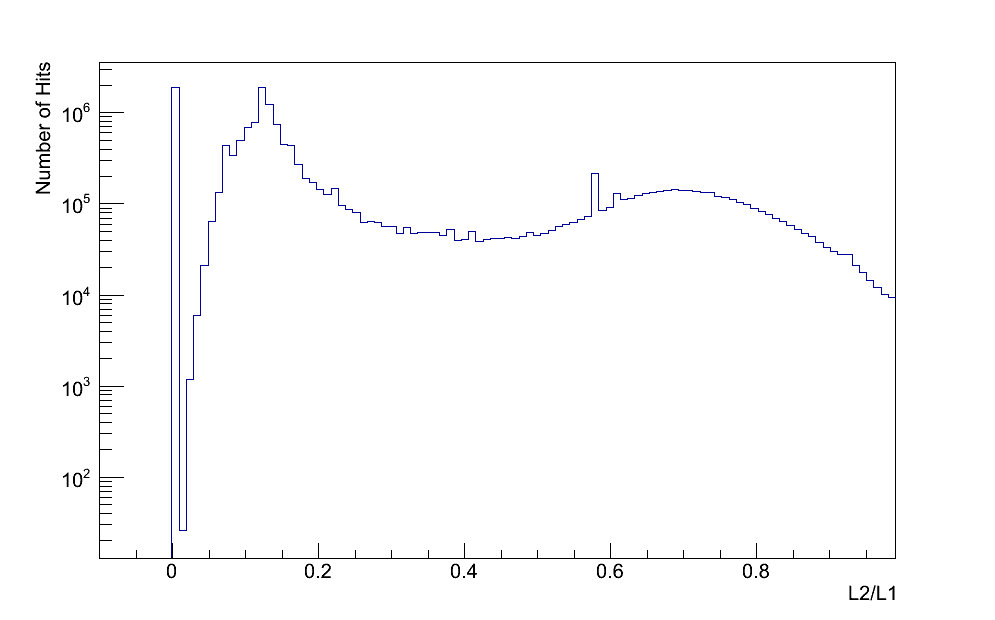
\includegraphics[width=1\textwidth]{Hits_Weight}

\caption{\label{fig:Ratio-of-L2/L1}Ratio of L2/L1 derived from PCA of neighbours
hits}


\end{figure}


\begin{figure}


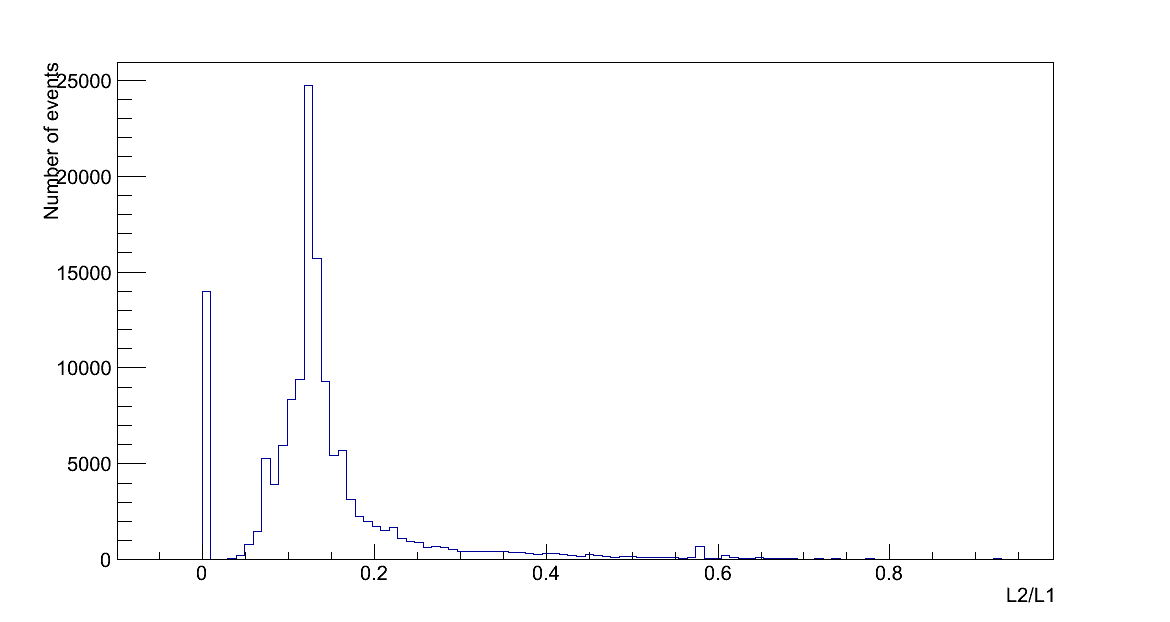
\includegraphics[width=1\textwidth]{Hits_Weight_track}

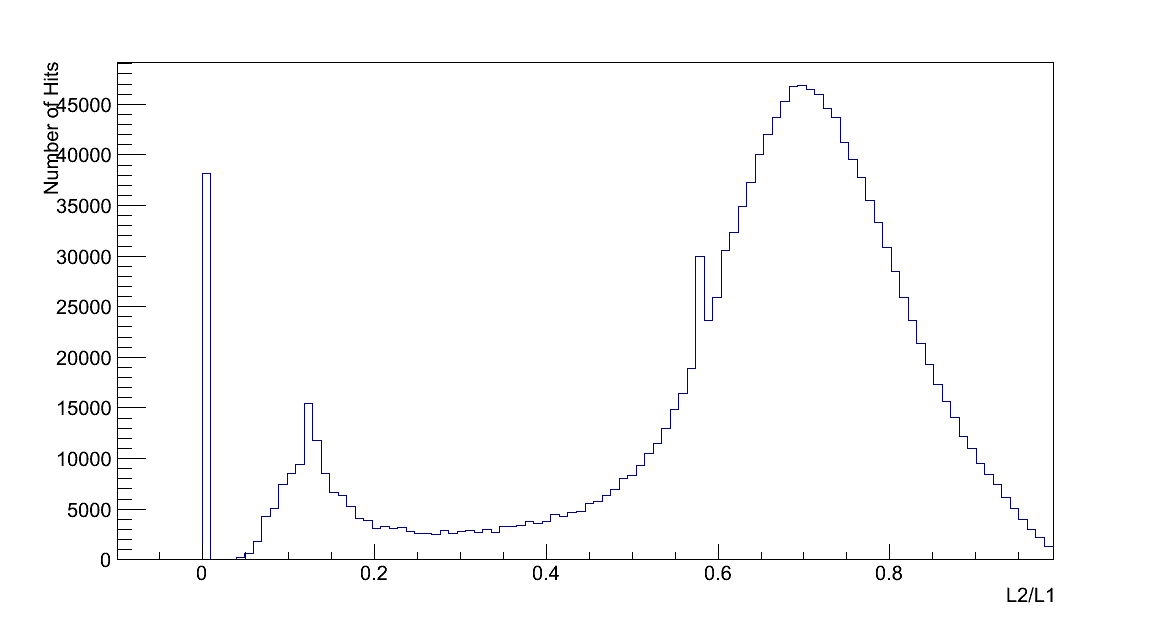
\includegraphics[width=1\textwidth]{Hits_Weight_shower}\caption{\label{fig:Ratio-of-L2/L1-track}Ratio of L2/L1 for preselected muon
tracks (top) and preselected showers (bottom) }
\end{figure}



\subsubsection{MIP tagging}

Once hits are sorted in thos three categories. Clusters are built
plane by plane by adding hits in plane distant from less than 4 cm
to an existing cluster. Two collections are built. ``Interaction''
clusters are built from CORE hits and ``real'' clusters from the
other hits. Finally ``Interaction'' clusters of less than 5 hits
are moved in the ``real'' collection and in paralell ``real''
clusters of more than 5 hits are moved in the ``interaction'' one.

The ``real'' collection is then used to reconstructed track segments
according to this algorithm:
\begin{itemize}
\item Once again principal component anlysis is used for all clusters to
find main direction in a 15 cm sphere around each point
\item Each point is associated to existing tracks according to

\begin{itemize}
\item if the track has at least 2 hits, the error of the extrapolation is
taken and the point is added if

\begin{itemize}
\item It is not the track path
\item it is less than 3 planes away from the end of the track
\item it is less than 5 sigma from the extrapolation
\end{itemize}
\item if the track has one hit

\begin{itemize}
\item the track hit is one plane before
\item the principal axis of the cluster is used to build track parameter
and point is added if it is less than 6 cm from the extrapolation
\end{itemize}
\end{itemize}
\item If no association is found, a new single hit track is created with
track parameters deduced from the principal component analysis of
its neighbouring.
\end{itemize}
The algorithm is run handling hits from the beam entry to the end
of the calorimeter. At the end , a last pass is done trying to associate
single hit tracks and previously unselected hits to valid segments.
Finally all hits belonging to a cluster associated to a track segment
is tagged MIP. The figure \ref{fig:60-GeV-Pion} shows the result
of the different steps of the algorithm.

\begin{figure}
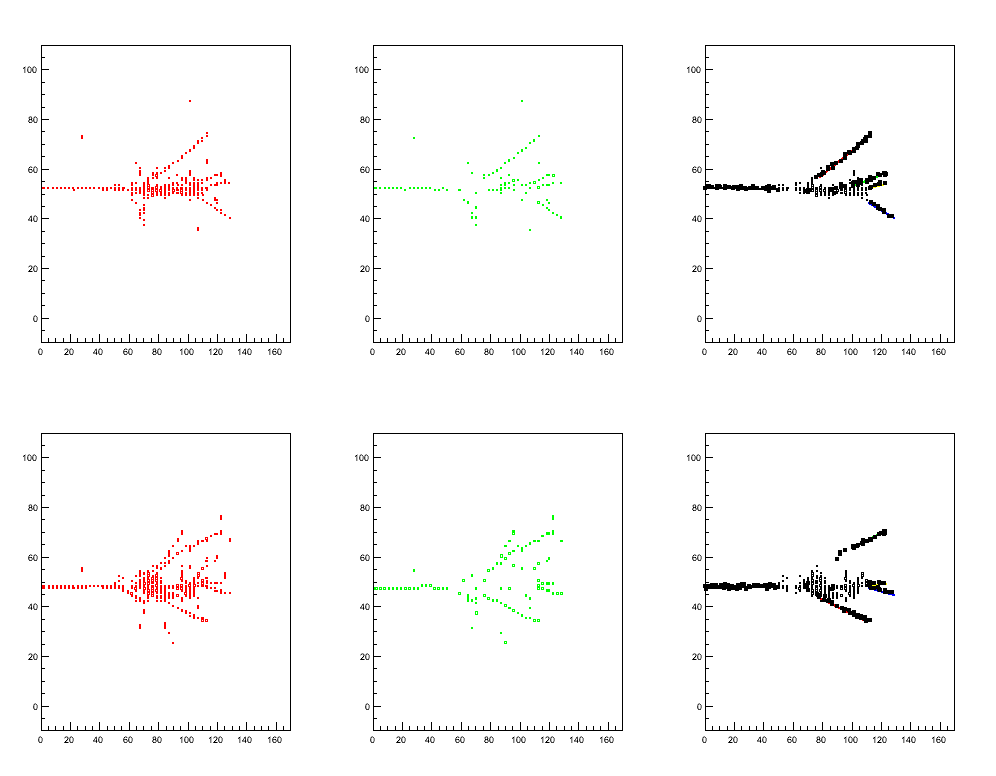
\includegraphics[width=1\textwidth]{60GevPion_MIP}

\caption{\label{fig:60-GeV-Pion}60 GeV Pion interaction display. The left
(red) column shows the hits position in (Z,X) and (Z,Y) projection.
The midle (green) column shows the ``real'' collection of clusters
projection. Finally on the right, track segments, MIP hits (black)
and 3D clusters of CORE hits are shown}
\end{figure}


The track segments can also be used to dicriminate muons and elctrons
from hadrons, using the ration of the total track length over the
total number of hits. The figure \ref{fig:Ratio-of-LOH} shows this
ratio. The peak at zero corresponds to electron with no MIP exiting
from the shower. The 1.4 peak is due to muons with a hit multiplicity
\textasciitilde{} 1.6 and finally hadron showers have a low ratio
up to 0.7. Events are tagged:
\begin{itemize}
\item ELECTRON if R<1E-4
\item MUON if R> 0.75
\end{itemize}
\begin{figure}
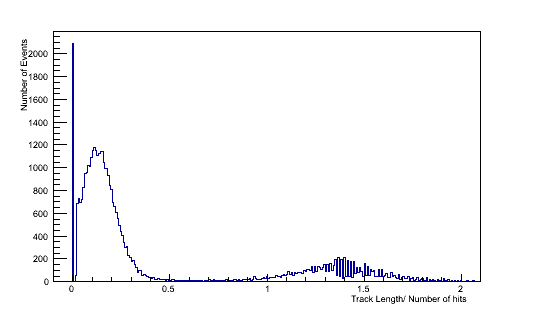
\includegraphics[width=1\textwidth]{TrackLength_Over_Hits}

\caption{\label{fig:Ratio-of-LOH}Ratio of total tracks length over the total
number of hits per event in a 60 Gev Pion run}


\end{figure}

\end{document}
